
\documentclass{beamer}
\usepackage{float}

\usetheme{default}

\title{Secure Shell(SSH)}

\author{Kiran Vasudev\inst{1}}

\institute[]
{
	\inst{1}
	Hochschule Bonn-Rhein-Sieg
	
}

\begin{document}
	
	\begin{frame}
	\titlepage
\end{frame}

\begin{frame}{Outline}
\tableofcontents
\end{frame}

\begin{frame}[allowframebreaks]{What is it?}
\section{What is it?}

	\begin{itemize}
		\item {
			A powerful software based approach to network security.
		}
		\item {
			Based on a client/server architecture.
		}
		\item{The SSH server program accepts/rejects connections to its host computer}
		
		\item{
			The SSH client program, running on other computers are used to make requests to the server.
		}
		\item{
			All communication between server and client are encrypted and hence are protected from any modifications.
		}
		\item{Better than non secure traditional architectures such as FTP and TELNET}
		
	\end{itemize}
	\begin{figure}
		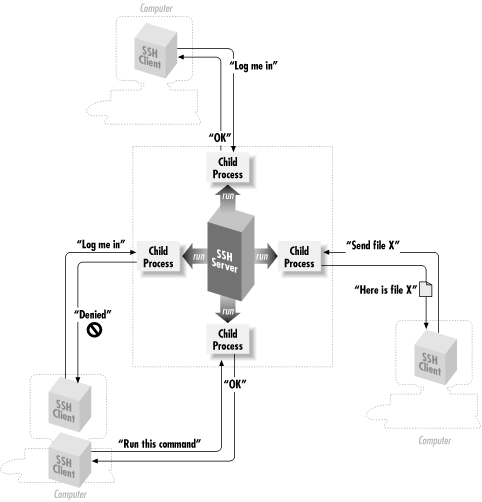
\includegraphics[scale=0.4]{images/arch}
		\caption{SSH Architecture\cite{arch}}
	\end{figure}
	


\end{frame}

\begin{frame}{What it is not}
\section{What it is not}
\begin{itemize}
\item {
It is not a true shell and hence does not provide a command history or command interpreter. A channel is created using SSH to run a shell on a remote computer.
}
\item {   
It is not a complete security solution. It still can be hacked.
}
\end{itemize}
\end{frame}

\begin{frame}{Why use SSH?}{}
\section{Why use SSH?}
\begin{itemize}
\item {
	Prevents interception of data between two systems.
}
\item {Tackles the problem where a nefarious computer impersonates a particular host.}
\end{itemize}
\end{frame}	

\begin{frame}{SSH in MAS}
\section{SSH in MAS}
\begin{itemize} 
	\item Use SSH to run processes on robots. Example: ROSMASTER
	\item Can also use SSH to access and clone repositories from GitHub
\end{itemize}
\end{frame}	


\begin{frame}{References}
\section{References}

\begin{thebibliography}{10}


\bibitem{arch}
\href{https://docstore.mik.ua/orelly/networking_2ndEd/ssh/ch01_01.htm}{SSH Architecture}




\end{thebibliography}
\end{frame}

\end{document}


